%\documentclass[a4paper,10pt]{article}
\documentclass[10pt]{article}
\usepackage[utf8]{inputenc}
\usepackage{xspace}
\usepackage{url}
\usepackage{graphicx,graphics} 
\usepackage{color}
\usepackage{amsmath}
\usepackage{amsfonts}
\usepackage{amssymb}
\usepackage{amsthm}
\usepackage{algorithm}
\usepackage{algorithmic}
\usepackage{longtable}
\usepackage{complexity}
\usepackage{tkz-graph}
\usepackage{float}
\usepackage{tabularx}
\usepackage{setspace}
\usepackage{icomma}
\renewcommand{\algorithmicrequire}{\textbf{Input:}}
\renewcommand{\algorithmicensure}{\textbf{Output:}}
\usepackage{authblk}
\usepackage[colorlinks=true,breaklinks=true,linkcolor=blue]{hyperref}


\newcommand\rmatching{${\cal R}$-matching\xspace}
\newcommand\mdelay{$\cal M$-delay\xspace}
\newcommand\matchedgraph{{\bf matched graph}}
\newtheorem{proposition}{Proposition}
\newtheorem{theorem}{Theorem}

\setlength{\parskip}{1ex} % Espace entre les paragraphes

\newtheorem{fact}{Fact}
\newtheorem{lemma}[theorem]{Lemma}
\newtheorem{definition}{Definition}
\newtheorem{corollary}{Corollary}

% \renewcommand{\thefootnote}{\*}

\newcommand{\todo}[1]{{\color{red} TODO: {#1}}}
\newcommand\pazl{\textsc{pazl}\xspace}
\newcommand\pall{\textsc{pall}\xspace}
\newcommand\bra{\textsc{bra}\xspace}
\newcommand\pra{\textsc{pra}\xspace}
\newcommand\minpra{\textsc{min-pra}\xspace}
%opening
\title{Deterministic Scheduling of Periodic Messages for Cloud RAN}
 

\author[1]{Dominique Barth}
\author[1,2]{Ma\"el Guiraud}
% \author[1]{Christian Cad\'er\'e}
 \author[2]{Brice Leclerc}
 \author[2]{Olivier Marc\'e}
\author[1]{Yann Strozecki}
\affil[1]{David Laboratory, UVSQ}
\affil[2]{Nokia Bell Labs France}

\begin{document}

\maketitle\section{Model and Problems}\label{sec:def}

We use the notation $[n]$ to denote the interval of $n$ integers $\{0,\dots,n-1\}$.

  \subsection{Discrete time model}
  In the model presented here, the time is discrete. The unit of time  is called a {\bf tic}. This is the time needed to transmit an atomic data of size $Q$ over the fastest link of the network. Since the speed of the links on the network can be different, the number of tics needed to transmit an atomic data through a link can be different depending on the link. In order to consider only integers, the fastest link of the network can be virtual if there is no link of speed equal to the least common multiple of the speeds of all links in the network. We denote by ${\cal S} = \{s_0,s_1,\ldots,s_n\}$ the set of speed of the links. The number of tics needed to send an atomic data of size $Q$ on a link $i$ is thus equal to $\frac{LCM({\cal S})}{s_i}$ tics, where $LCM({\cal S})$ is the Least Common Multiple of the set {\cal S}. Figure~\ref{fig:datagram} illustrates this phenomenon.
  
  \begin{center}
  
  \begin{figure}
  \begin{minipage}[b]{0.50\linewidth}
  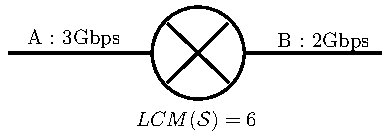
\includegraphics[width=0.8\textwidth]{links.pdf}
  \end{minipage}
\hfill
  \begin{minipage}[b]{0.50\linewidth}
    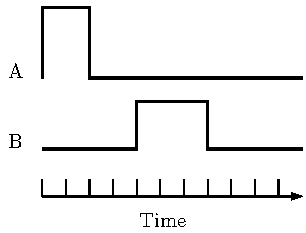
\includegraphics[width=0.8\textwidth]{chronotics.pdf}
  \end{minipage} 
  \caption{Different number of tics used to carry an atomic data of size $Q$}
  \label{fig:datagram}
 \end{figure}
 
    \end{center}
  \subsection{Network modeling}
  
The network is modeled as a directed graph $G=(V,A)$. The \textbf{sending tic} of a message in a vertex $u$ is the tic at which the beginning of this message is sent from $u$. Also, the \textbf{reception tic} of a message in a vertex $v$ is the tic at which the beginning of the message arrives in $v$.  Each arc  $(u,v)$ in $A$ is labeled by an integer weight $\Omega(u,v)$ which represents the number of tics elapsed between the sending tic of the message in $u$ and the reception tic of this message in $v$ using this arc. A {\bf route} $r$ in $G$ is a directed path, that is, a sequence of adjacent vertices $u_0, \ldots , u_{l}$, with $(u_i,u_{i+1}) \in A$.  The {\bf weight of a vertex} $u_i$ in a route $r=(u_0,\dots,u_l)$ is defined by $\lambda(u_i,r)= \sum\limits_{0 \leq j <i} \Omega(u_j, u_{j+1})$. It is the number of tics needed between the sending tic of a message in the first vertex of the route and the reception tic of this message at $u_i$. We also define $\lambda(u_0,r)=0$. The weight of the route $r$ is defined by $\lambda (r)= \lambda (u_l,r)$.
We denote by $\cal R$ a set of routes, the pair $(G,\cal R)$ is called a {\bf routed network} and represents our telecommunication network.
The first vertex of a route models an antenna (RRH) and the last one a data-center (BBU) which computes an answer to the messages sent by the antenna.

   \subsection{Messages dynamic}
	 
    %Time is discretized, hence the unit of all time values is a, the time needed to transmit a minimal unit of data over the network. \todo{parler des différents débits et de ce que ça change}. The weight of an arc is also expressed in tics, that is the time needed by a message to go through this arc.
    
        In the process we study, some {\bf datagrams} are sent on each route. The size $|d|$ of a datagram $d$ is an integer, correspond to the number of atomic data needed to carry the information contained by the datagram. The number of tics needed by a node $u$ to emit the datagram through the link $(u,v)$ of speed $s_i = {\cal S}(u,v)$ is denoted $|d|_{(u,v)}$ and has for value $ |d| \times \frac{LCM({\cal S})}{s_i}$ . Once a datagram have been emitted, it cannot be fragmented during its travel in the network. Thus, due to the different speed of the links, when the beginning of a datagram $d$ arrives in a node $u$ of a route $r$, it might be delayed in the node to avoid the fragmentation of the datagram. The number of tics lost in the node is given by the function $l(d,u,r)$.\\
        \begin{lemma}
        If a datagram $d$ arrives at a node $v$ through the link $(u,v)$ of speed $s_i$, and must be sent back in the link $(v,w)$ of speed $s_j$, then l(d,v,r) is equal to $ \max( 0, |d|_{(u,v)} - |d|_{(v,w)} )$ tics.
        \end{lemma}
        \begin{proof}
        We consider a buffer in the node $v$. If $t$ is the reception tic of the datagram $d$ in $v$, it has fully reach the buffer in $|d|_{(u,v)}$ tics that is, at date $t+|d|_{(u,v)}$. If the datagram is fully contained in the buffer, the node can send it in $|d|_{(v,w)}$ tics. We want to choose the sending tic such that the datagram will not be fragmented.\\
        If $s_i \geq s_j$, the buffer fills as fast or faster as it empties, thus, the datagram crosses the node without additional delay.\\
   
        If $s_i < s_j$, we want to wait the time at which the datagram can be re-sent without fragmentation. The last tic time at which the node receive some data is $t+|d|_{(u,v)}$. Thus, the next tic ($t+|d|_{(u,v)}+1$), is the minimum date at which the node can send the end of the datagram on the link $(v,w)$. Since the node needs $|d|_{(v,w)}$ to completely send the message, it can start to emit at date $t+|d|_{(u,v)}+ 1 - |d|_{(v,w)}$. 
        \end{proof}
        
          Let $r=(u_0,\dots,u_l)$ be a route. In order to avoid the contention, one can choose to buffer a datagram $d$ in any node $u_i$ of the route. The function $b(d,u_i), i \in \{0,\ldots,l\}$ associate to each couple datagram-node an integer. Those integers represent the buffering time of the datagram in each nodes of the route. For all $i$, $b(d,u_i) \in \mathbb{N}$.
              
The \textbf{departure time} of a datagram $d$ on a route $r$, denoted by $\theta_r(d)$, is the sending tic of $d$ at node $u_0$, the first vertex of $r$. 
 Also, the \textbf{reception time} of this datagram $d$ at a vertex $u_i$ in $r$, i.e. the first tic at which the datagram sent at time $\theta_r(d)$ on $r$ reaches $u_i$, is $t(d,u_i,r) = \theta_r(d) + \lambda(u_i,r) + \sum_{k=0}^{i-1}( b(d,u_k) + l(d,u_k,r))$. In other words, the date at which a datagram to reach a vertex $u_i$ correspond to the date of the emission of this datagram in the RRH, plus the physical delay of the links, plus the buffers induced by the physical constraints of the network, or determined by the logical solutions proposed.
   
        A {\bf stream} $S$ is a sequence of several datagrams. To each route of the routed network is associated a stream. The cardinal of a stream, denoted $\#S$ is the number of datagrams in the stream. Let us consider a stream $S_i$ on the route $r_i$, the datagrams $\{d_0,\ldots,d_{\#S_i-1}\}$ are sent in sequence from the first node of the route, that is : $\theta_{r_i}(d_0) < \theta_{r_i}(d_1) < \ldots < \theta_{r_i}(d_{\#S_i-1})$ .  \\
       For each route, the size of a stream is $\sum_{i=0}^{{\#S-1}} |d_i|$ . The amount of data sent by an RRH to its BBU is the same, regardless of the route. Hence, we assume that this size is the same for all route, and we denote it by $\tau$. 
        
          
       Let us call $[t(S,u,r)]$ the set of tics used by a stream $S$ on a route $r$ in the arc $(u,v)$, that is $[t(S,u,r)] =  \bigcup_{i=0}^{\#S -1} \{t(d_i,u,r) + i \mid 0 \leq i < |d_i|_{(u,v)}\}$.
      Let $r_1$ and $r_2$ be two routes, on which two streams $S_1$ and $S_2$ are sent.
      We say that the two routes have a {\bf collision} if they share an arc $(u,v)$ and $[t(S_1,u,r_{1})] \cap [t(S_2,u,r_{2})] \neq \emptyset$.
            
   In the context of cloud-RAN applications, we need to send a stream from an RRH $u$ to a BBU $v$ and then 
      we must send the answer from $v$ back to $u$. We say that a routed network $(G, {\cal R})$ is \textbf{symmetric} if the set of routes is partitioned into the sets $F$ of \textbf{forward routes} and $B$ of \textbf{backward routes}. There is a bijection $\rho$ between $F$ and $B$ such that for any forward route $r \in F$ with first vertex $u$ and last vertex $v$, the backward route $\rho(r) \in B$ has first vertex $v$ and last vertex $u$. In all practical cases the routes $r$ and $\rho(r)$ will be the same with the orientation of the arcs reversed, which corresponds to bidirectional links in \emph{full-duplex} networks, but we do not need to enforce this property.

     
     We now describe the process of the sending of a stream and of its answer. First, the datagrams of a stream $S_r$ are sent at $u$, through the route $r \in A$, at times $\{\theta_r(d_0),\ldots,\theta_r(d_{\#S_r-1}) \}$.
      Those datagrams are received by $v$, i.e., the last vertex of $r$ at times $\{t(d_0,v,r),\ldots,t(d_{\#S_r-1},v,r)\}$. 
     Once $v$ has received all the datagrams of a stream, the answer is computed and sent back in a stream $S_{\rho_r}$. Note that $\#S_{\rho_r}$ may be not equal to $\#S_r$, i.e. the answer is not necessarily under the same form as the initial stream. Then, the node $v$ send $S_{\rho_r}$ to  $u$ on the route $\rho_r$ at times $\{\theta_{\rho_r}(d_0),\ldots,\theta_{\rho_r}(d_{\#S_{\rho_r}-1}) \}$.

     Note that, in the process we describe, we do not take into account the computation time a BBU needs to deal with one message. It can be encoded in the weight of the last arc leading to the BBU and thus we do not need to consider it explicitly in our model. 

      We define the {\bf full reception time} of a stream $S_r$ on a node $v$ through the link $(u,v)$ by $rt(S_r,v) =  \displaystyle \max_{i \in \{0,\ldots,\#S_r-1\}} ( t(d_i,v,r) + |d_i|_{(u,v)} )$. This is the time at which the end of the last datagram of the stream has reach the vertex $v$. Recall that a BBU needs to completely receive a message before sending of the answer, that is $rt(S_r,v)  < \theta_{\rho_r}(d_0)$
      

      The whole process time for a route $r$ is equal to $PT(r)= rt(S_{\rho_r},u) - \theta_r{d_0} $, where $u$ is the RRH.      
      In the process time, we count the time between the time the first tic of the stream is emitted and the time at which the last tic of the answer comes back. 
      Each route must respect a time limit that we call \emph{deadline}. To represent these deadlines, 
     we use a deadline function $d$, which maps to each route $r$ an integer such that $PT(r)$ must be less than $d(r)$.
  

        An {\bf assignment} of a routed network $(G,\cal R)$ is a function that associates to each datagram of each route its departure time and its buffers. In an assignment, \emph{no pair of routes has a collision}.
	 
      We consider the following decision problem.

      \noindent {\bf Periodic Assignment for Low Latency (\pall)} 

      \noindent {\bf Input:}  A symmetric routed network $(G,{\cal R})$, the integers $P$, a deadline function $d$ and a set of streams.
      
      \noindent {\bf Question:} does there exist an assignment $m$ of $(G,{\cal R})$ such that for all $r \in {\cal R}$, $PT(r) \leq d(r)$?


\bibliographystyle{ieeetr}
\bibliography{Sources}

\end{document}
